% !TEX root = main.tex
\section{Methods} % (fold)
\label{sec:methods}

\subsection{Producing the fragment PDB file}
The NMR structure of 4EBP2 used in this project is the same as in Bah \textit{et al.}
and has PDB ID \href{http://www.rcsb.org/pdb/explore/explore.do?structureId=2MX4}{\textcolor{blue}{2MX4}}.
Because 2MX4 includes 62 residues, we chose to simulate only a portion of the protein centered around one of the phosphorylated threonines, T37.
The full structure includes two known phosphothreonine sites, T37 and T46.
The fragment used in the simulations includes two residues before T37 and six after, comprising a nonamer with the sequence CTTPGTLF.
It extends to both ends of the loop in which T37 resides, as seen in Figure~\ref{fig:2MX4}.

\begin{figure}[h!]
  \caption{2MX4 in PyMOL. The fragment containing T37 used in the simulations is highlighted in green sticks.}
  \centering
    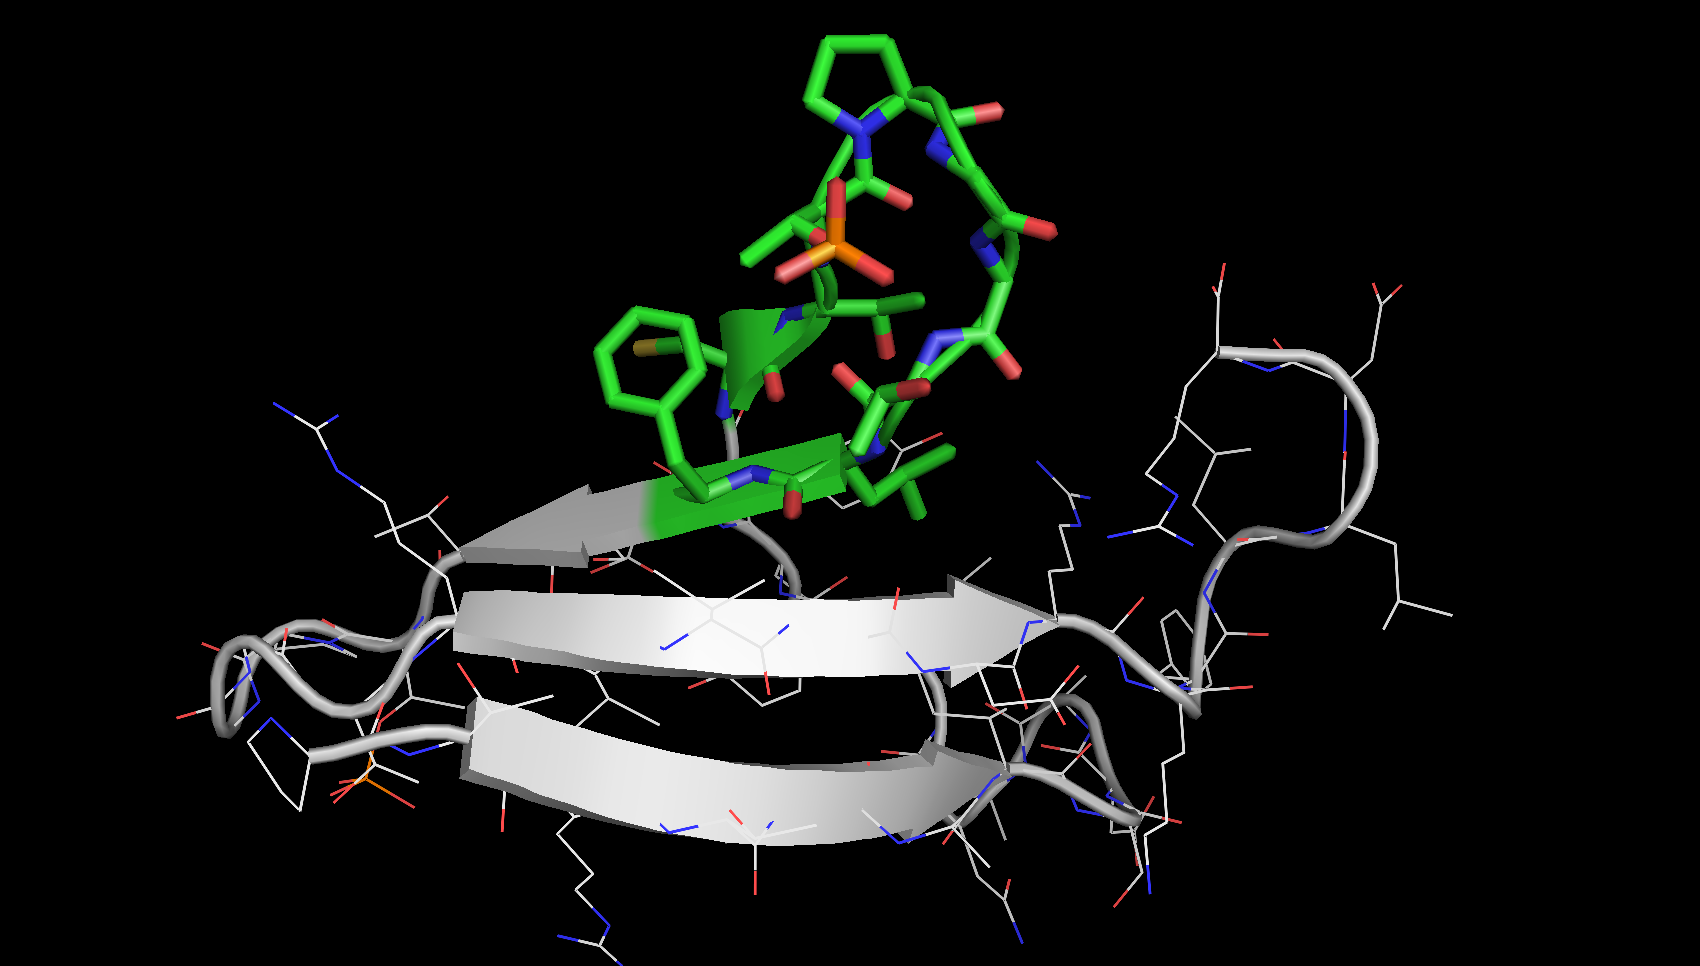
\includegraphics[width=0.5\textwidth]{2MX4}
  \label{fig:2MX4}
\end{figure}

\subsection{Capping the terminii}
Because the fragment does not have the same terminii as a native peptide, we capped the ends to mitigate unrealistic interactions.
For all versions of the fragment simulated, the N-terminus was acetylated and the C-terminus was methylamidated.
These caps were added with \texttt{psfgen} using the ACE and CT2 modifications on the N- and C-terminus, respectively.

\subsection{Dephosphorylating the fragment}
The dephosphorylated version of the fragment was created by removing the phosphate ion from the original, phosphorylated fragment.
\texttt{VMD}'s autopsf tool automatically added a hydrogen to the hydroxyl group of the unphosphorylated T37.

\subsection{Creating the extended versions of the fragment}
We used PyRosetta to generate an extended fragment with the same sequence as the NMR structure, CTTPGTLF.
To create an extended fragment with a phosphorylated threonine, we used the patch functionality of \texttt{psfgen}.
Because the bond lengths of the phosphate ion in the patched phosphothreonine were not generated correctly,
we ran 1000 steps of minimization before all simulations involving this extended fragment so that the oxygen atoms could adjust to their natural positions.

\begin{figure}[h!]
  \caption{The phosphorylated, extended fragment in PyMOL. Note the improper bond lengths in the phosphate ion that must be related with minimization.}
  \centering
    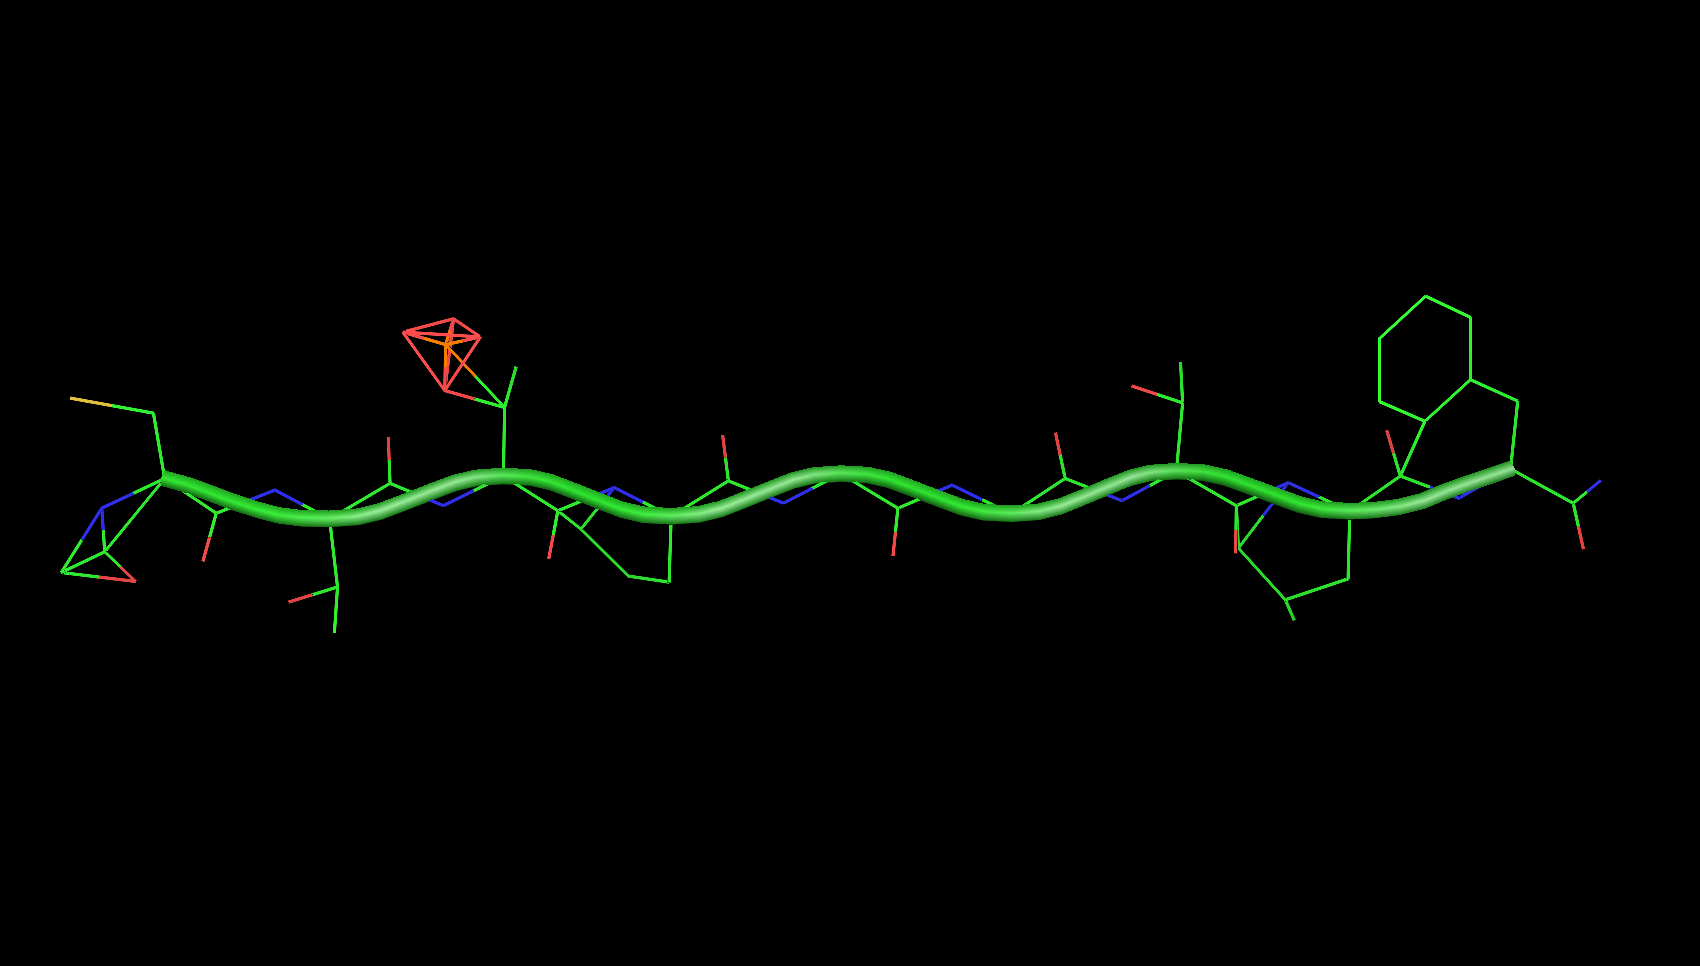
\includegraphics[width=0.5\textwidth]{2MX4_p1_extended}
  \label{fig:2MX4_p1_extended}
\end{figure}

\subsection{Generating the PSF files}
We generated PSF files using either the \texttt{psfgen} command-line tool or \texttt{VMD}'s autopsf, depending on our needs.
Phosphothreonine requires additional topology and parameter files in addition to the standard protein ones.
The complete list of topology files given to \texttt{psfgen} is given below in the order we used when generating PSF files:
\begin{itemize} \itemsep 1pt
  \item top\_all36\_prot.rtf
  \item top\_all36\_na.rtf
  \item toppar\_all36\_prot\_fluoro\_alkanes.str
  \item toppar\_all36\_prot\_na\_combined.str
\end{itemize}
Because we could not get \texttt{VMD}'s autopsf tool to properly patch threonine into phosphothreonine, we used \texttt{psfgen} for the phosphorylated fragments.
The files and scripts used for PSF file generation can be found in the \texttt{psfgen} directory of the repository.

\subsection{Solvating the fragments}
All fragments were solvated using \texttt{VMD}'s solvation box tool before they were simulated.
We tried solvation boxes of size 8\AA, 10\AA, and 12{\AA} since we did not know exactly how much solvent was required to avoid wrap-around effects.
The fragments were rotated to minimize volume.

\subsection{File naming conventions}
Because we generated so many different versions of the fragment, we adopted consistent naming conventions for the files.
The first part of each file is \texttt{2mx4},
the second is which sites are phosphorylated (\texttt{p1} means that T37 is phosphorylated, \texttt{up1} means it is not),
the third is an optional \texttt{extended} keyword indicating that the fragment is extended,
and for solvated files there is a fourth part that indicates the size of the solvation box (\texttt{s8} means an 8{\AA} solvation box).
For the free energy perturbation simulations, there is a fifth part for alchemical files, \texttt{alch}, and for fixed files, \texttt{fixed}.

\subsection{TCL parameters}
The TCL parameters for the \texttt{NAMD} simulations remain largely unchanged from those introduced in class.
Each step was a femtosecond and energies were printed every 100 steps.
Simulations were minimized for 1000 steps.
Each simulation ran for a different amount of time depending on cluster availability and time constraints.

% section methods (end)
